\section{Boundary preserving TetGen comparison}\label{app:tetgen}

\begin{figure}
    \centering
    \parbox{0.02\linewidth}{~}\hfill\hfill
    \parbox{.47\linewidth}{\centering Mean}\hfill
    \parbox{.47\linewidth}{\centering Max}\par
    %%%%%
    \parbox{0.02\linewidth}{\centering\rotatebox{90}{\scriptsize{Model Count}}}\hfill\hfill
    \parbox{.47\linewidth}{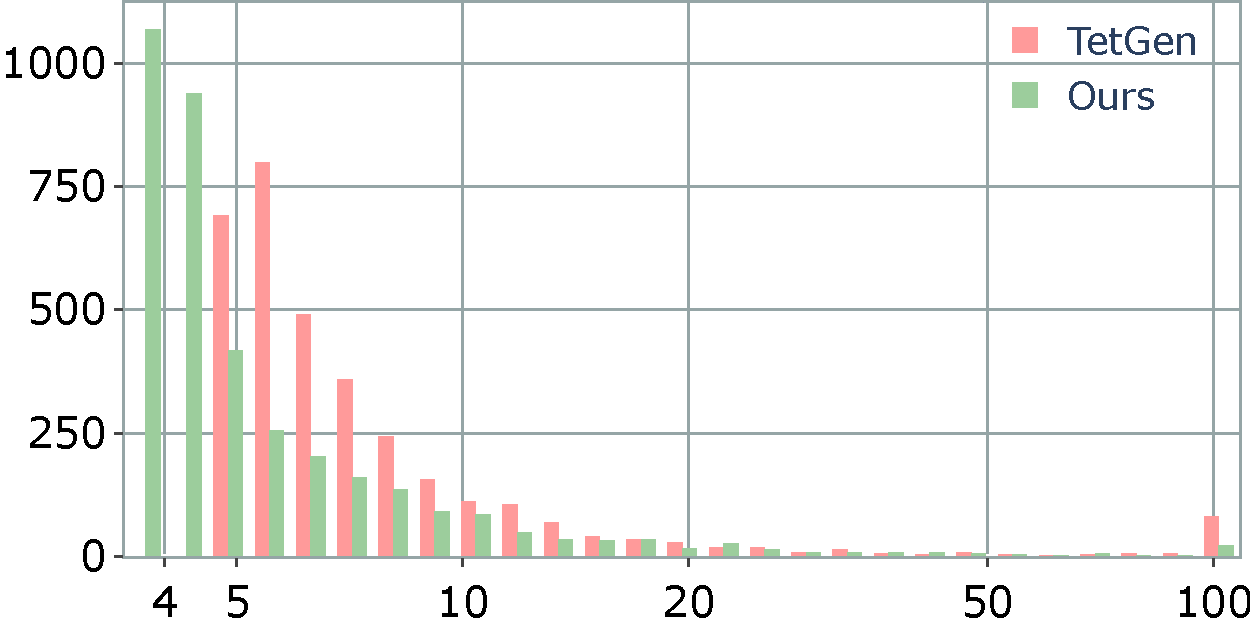
\includegraphics[width=\linewidth]{curve_meshing_in_shell_tex/figs/stats/tetgen_meanE}}\hfill
    \parbox{.47\linewidth}{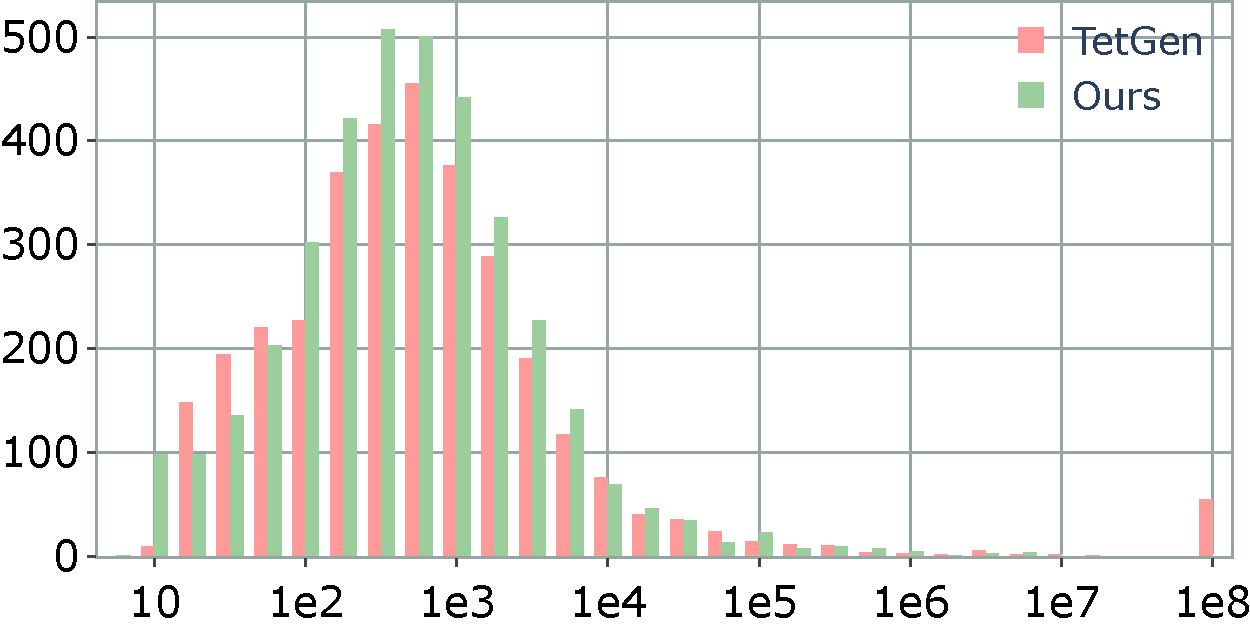
\includegraphics[width=\linewidth]{curve_meshing_in_shell_tex/figs/stats/tetgen_maxE}}\par
     \scriptsize{AMIPS Energy}
    \caption{Histogram of mean and maximum conformal AMIPS energy~\cite{Rabinovich:2017} of the output of our method and TetGen.}
    \label{bichon:fig:energy-max-avg}
\end{figure}

\begin{figure}
    \centering
    \parbox{.7\linewidth}{\centering
    \parbox{0.02\linewidth}{\centering\rotatebox{90}{\scriptsize{Model Count}}}\hfill
    \parbox{.95\linewidth}{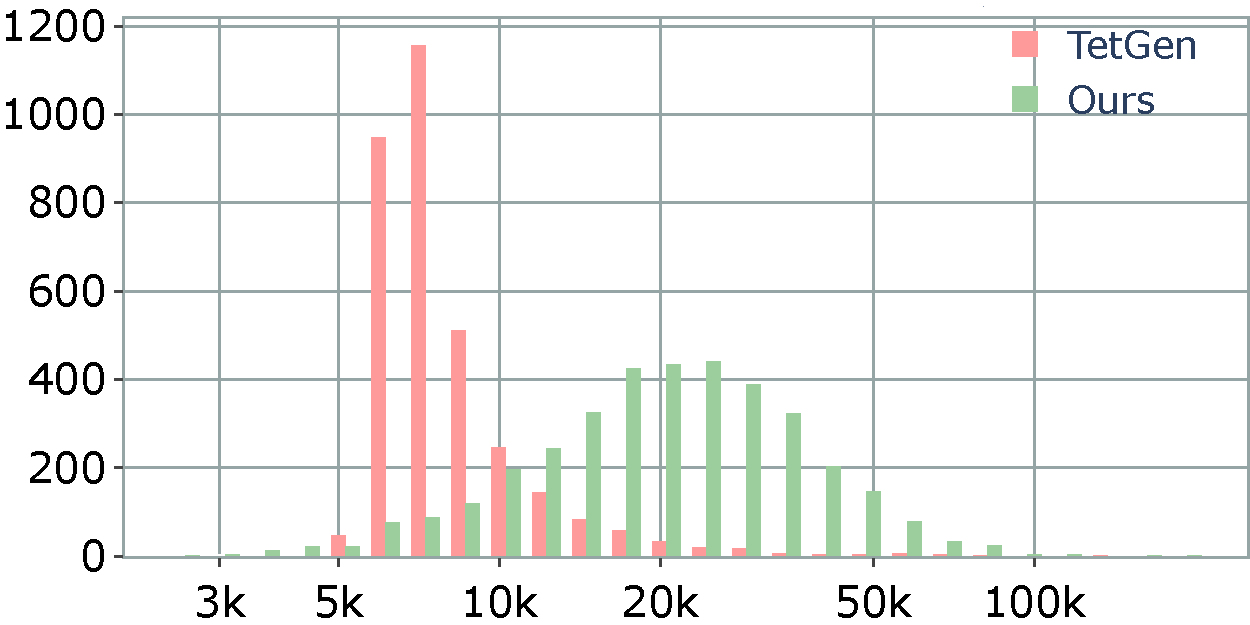
\includegraphics[width=\linewidth]{curve_meshing_in_shell_tex/figs/stats/tetgen_TO}}\par
    \scriptsize{Tetrahedra Number}
    }
    \caption{Histogram of output tetrahedra number for TetGen and {our} method. }
    \label{bichon:fig:numt}
\end{figure}

We compared our conforming tetrahedral meshing algorithm (Section~\ref{cumin:sec:tets}) with TetGen on the linear shells (triangle meshes) of 3522 models from the Thingi10k dataset, giving each model sufficient computing resources (2 hours maximum running time and 32GB memory usage). Inheriting the robustness from TetWild, our method successfully processed all the inputs while preserving the triangulation, while TetGen fails on 224 models (215 models are not conforming, and 9 models have no output).

% \ZZ{about the tail, tetgen meanE.max = 3e8, ours meanE.maxE = 3e5  tetgen maxE.max = 3e12, ours meanE.maxE = 7e6, all truncated}

In Figure~\ref{bichon:fig:energy-max-avg}, we show the average and maximum element quality of the output of our method and TetGen. Our method has {a} better average and maximum output quality than TetGen. Note that in the quality plot, the ``tail'' of TetGen's distribution is longer than ours. The maximum average energy of TetGen's output and ours are $3\times 10^8$ and $3 \times 10^5$ respectively. The largest maximum energy of TetGen's output and ours are $3\times 10^{12}$ and $7 \times 10^6$ respectively. Our method generates denser output (Figure~\ref{bichon:fig:numt}), but our focus is on robustness instead of efficiency in this step.

